\documentclass[cn,10pt,math=newtx,chinesefont=founder]{elegantbook}

\title{振動與波}
\subtitle{2021年}

\author{李宥頡}
\institute{National Taiwan University}
%\date{May 2, 2021}
%\version{4.1}
%\bioinfo{自定义}{信息}


\setcounter{tocdepth}{3}

%\logo{logo-blue.png}
\cover{cover.jpg}

% 本文档命令
\usepackage{array}
\newcommand{\ccr}[1]{\makecell{{\color{#1}\rule{1cm}{1cm}}}}

\definecolor{customcolor}{RGB}{32,178,170}
\colorlet{coverlinecolor}{customcolor}

\begin{document}

\maketitle
\frontmatter

\chapter*{序}
物理學家習慣按照物質運動的型態,把古典物理分成力學,熱學,電學,光學等子學科。然而某些形式的運動是橫跨所有
這些學科的,其中最典型的就是振動與波。在力學方面有力學波,在電磁學有電磁震盪和電磁波,甚至到了近代物理中更是
延伸出物質波的概念,接續發展的量子力學也是以薛丁格波方程(Schrödinger Equation)為中心的波動力學。以上種
種都表明,振動與波在物理的重要性,可惜的是在目前中學物理的課程安排下,由於缺乏相關的數學基礎,並不能延伸更多
概念,故此講義將會循序漸進,透過基本微分方程的介紹切入到各種振盪。本書內容主要參考以下幾本書籍,並會以此處的
縮寫為主。
\begin{itemize}
    \item 赵凯华, et al. 新概念物理教程——力学 (第二版). 北京: 高等教育出版社, 2004. (新概念力學)
    \item 程稼夫. "中 学 奥 林 匹 克 竞 赛 力 学 篇." 第 二 版. (程力)
    \item 舒幼生. "物理类: 力学." (2005). (舒力)
    \item Halliday, David, Robert Resnick, and Jearl Walker. Fundamentals of physics. John Wiley \& Sons, 2013. (Halliday)
    \item Kittel, Charles. Mechanics Berkeley Physics Course Vol 1. Tata Macgrawhill Publishing Company, 1965.
    \item Crawford, Frank S. Berkeley physics course: Waves. New York, NY, USA: McGraw-Hill, 1968.
\end{itemize}
\tableofcontents

\mainmatter

\chapter{基本知識}
\section{物理學中的微分}
運動學(Kinetics)涉及質點與物體的運動,我們主要關注物體的位置、速度、加速度等物理量隨時間的變化。在描述一個物理系統時,需要有對應的座標系,
最常見的為笛卡爾座標(Cartesian Coordinate),也就是以相互正交的座標軸x,y,z形成座標系。所謂運動方程(Equation of motion)即為給定任意時間t,
可知對應的位置(x,y,z),以下內容先以一維的直線運動為例,我們將探討運動學中的微分。


\section{微分方程}

\section{泰勒展開Taylor Expansion}

\section{位能曲線}
位能曲線是討論物體在保守力場中運動的重要工具,我們知道,位能是位置的函數,即
\begin{equation}
    U = U(\vec{r})
\end{equation}
在一維情況下為
\begin{equation}
    U = U(x)
\end{equation}
因此若我們做$U-x$圖,此圖能給我們許多重要的訊息,以下將一一介紹。
\begin{enumerate}
    \item 根據位能的定義,負的保守力作功為位能變化量,即$W_{con}=-\Delta U$,若取無窮小位移$dx$,則應有以下關係
    \begin{equation}
        F_{con} dx = -dU
    \end{equation}
    或是也可以解釋成保守力的定義為,負的位能對位置微分
    \begin{equation}
        F_{con} = - \frac{dU}{dx}
    \end{equation}
    故在$U-x$圖中,曲線的負斜率為保守力,斜率的絕對值越大,代表所受保守力的量值越大。
    \item 在$U-x$圖中做水平線,代表總能量為$E$,由於在此書大部分情況並沒有其他能量的出現,因此$E$也可以認為是力學能(動能加位能)。代表
    $E$的水平線減去對應位置$x$下的位能$U$,即為動能$E_k$。
    動能的公式$E_k = \frac{1}{2}mv^2$代表物體運動的劇烈程度,由公式可知,動能不可能為負值。因此若水平線$E$低於位能曲線之處,代表具有該能量$E$的
    物體不可能到達此位置,此概念就是力學中十分重要的位能井(Potential Well)。
    \item 位能曲線的局部最低點,也就是微積分所說的極小值(local minimum),在微積分裡極值可能發生在一次微分為零的地方,也就是$ \frac{dU}{dx} = 0$
    ,所以此處所受的保守力亦為零,相當於合力為零,根據牛頓定律,應處在靜止或等速直線的平衡狀態。對微積分比較有感覺的同學應該此時會有疑問,一次微分為零的位置
    也有可能對應到位能最大值,那該怎麼處理?我們知道對於物體的平衡,可以分成三種,穩定平衡(Stable Equilibrium),不穩定平衡(Unstable Equilibrium),
    以及隨遇平衡(Neutral Equilibrium),其判別法在中學課本中為,若給一個偏離其平衡位置不遠的位移,觀察物體是否能回到平衡位置。若能回到原平衡位置,即
    為穩定平衡,若不能,為不穩定平衡,最特殊的為隨遇平衡,物體會在其他位置建立新的平衡。以位能的角度其實就是在平衡的條件下($ \frac{dU}{dx} = 0$),討論
    二次微分$\frac{d^2 U}{dx^2}$的值,若$\frac{d^2 U}{dx^2}>0$,此處為位能極小值,代表附近的位能都比此處高,簡單畫附近的切線,可知偏離平衡位置的力會
    使物體傾向回到平衡位置。若$\frac{d^2 U}{dx^2}<0$,此處為位能極大值,代表附近的位能都比此處低,簡單畫附近的切線,可知偏離平衡位置的力會
    使物體離開原有的平衡位置。若$\frac{d^2 U}{dx^2}=0$或是不存在,即為隨遇平衡。由於在振動裡面我們需要探討的運動多為穩定平衡下的振盪,代表我們著重
    在可以回到原平衡位置的運動。
    \item 振動主要發生在位能極小值附近。結合上述的第二第三點,我們可以發現在給定一水平線E時,位能極小值同時代表動能極大值,當物體向逐漸遠離位能極小值時,
    會受到一反向的保守力(由切線可知),使物體動能減少,位能增加,此過程持續到所有能量轉化成位能,動能此時為零,相當於運動的折返點,便會折回位能極小處,
    以此方式來回振動。

\end{enumerate}




\section{例題}
%例題2
\begin{example} 
    水面上浮沉的木塊是在作簡諧振動嗎?如果是,其周期為多少?
    
    \rightline{[2]}
    
\end{example}

\begin{solution}
是簡諧振動,其周期為$T = 2\pi \sqrt{\frac{m}{S\rho_水g}}$。
\end{solution}

\begin{figure}[htbp]
\flushright
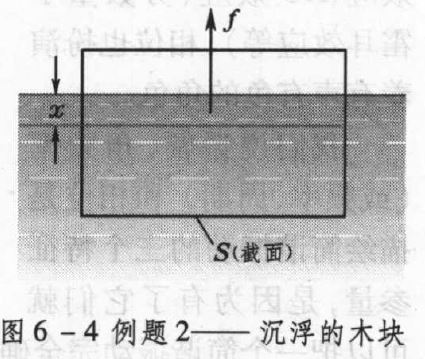
\includegraphics[width=0.4\textwidth]{image/6-4-2.JPG}
\end{figure}

\newpage


%例題3
\begin{example} 
    如圖6-5所示,勁度係數為k﹑質量為M的彈簧振子靜止地放置在光滑的水平面上,一質量為m的子彈以水平速度$v_1$射入M中,與之一起運動。選m﹑M開始共同運動的時刻為$t=0$,求固有角頻率﹑振幅和初相位。
    
    \rightline{[3]}
    
\end{example}

\begin{solution}
固有角頻率$\omega_0 = \sqrt{\frac{k}{M+m}}$,振幅$A = \sqrt{\frac{m^2}{k(M+m)}}v_1$,初相位$\varphi_0 = \pi/2$。
\end{solution}

\begin{figure}[htbp]
\flushright
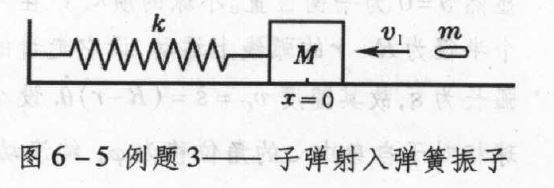
\includegraphics[width=0.5\textwidth]{image/6-5-3.JPG}
\end{figure}

\newpage


%例題4
\begin{example} 
    如圖6-6所示,在一勁度係數為k的彈簧下面掛一個質量為M的水桶,以振幅$A_0$上下振動。水桶底上有一小洞,水慢慢從中向外滲出。當水桶從上向下經過平衡點時,一滴質量為m的水大到表面張力不能支撐的地步而滴落下來。求此後水桶的運動情況。
     
    \rightline{[4]}
    
\end{example}

\begin{solution}
水滴滴落後水桶仍作簡諧振動,不過它的角頻率由$\omega_0=\sqrt{k/M}$變為$\omega = \sqrt{k/(M-m)}$,新平衡位置在原來之上距離為$mg/k$的地方。\\
取x軸向上,設水滴滴落後水桶的震動為$x = Acos(\omega t + \varphi_0)$,取水滴滴落的時刻為$t=0$,則在此時$x = Acos\varphi_0 = -mg/k$,$\Dot{x} = -\omega Asin\varphi_0 = -\omega_0 A_0$。\\
由此得$A = \sqrt{{(\frac{mg}{k})}^2 + {(\frac{\omega_0}{\omega}A_0)}^2} = \sqrt{{(\frac{mg}{k})}^2 + \frac{M-m}{M}{A_0}^2}$,$tan\varphi_0 = -\frac{kA_0}{mg}\sqrt{\frac{M-m}{M}}$。\\
從$tan\varphi_0 < 0$﹑$cos\varphi_0 < 0$和$sin\varphi_0 > 0$知$\varphi_0$應在第二象限。
\end{solution}

\begin{figure}[htbp]
\flushright
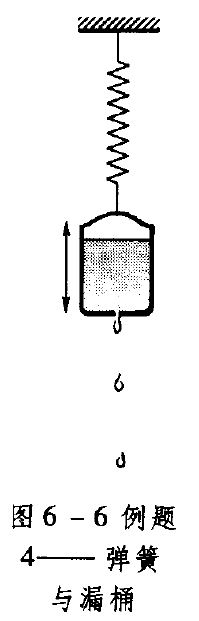
\includegraphics[width=0.2\textwidth]{image/6-6-4.JPG}
\end{figure}

\newpage


%例題5
\begin{example} 
    \begin{enumerate}[label=(\arabic*)]
    \item 圖6-7為一個線形三原子分子$A_2B$的模型。假定相鄰原子之間的結合力是彈性力,它們正比於原子的間距,求分子可能的縱向運動形式和相應的振動角頻率。
    \item $CO_2$分子的兩個振動縱模的頻率分別是$3.998x10^{13}$Hz和$7.042x10^{13}$Hz,試求CO鍵的彈性勁度係數k。原子質量單位$u = 1.660x10^{-27}$kg,碳的原子量=12,氧的原子量=16。
    \end{enumerate}
     
    \rightline{[5]}
    
\end{example}

\begin{solution}
\begin{enumerate}[label=(\arabic*)]
\item ${\omega_1}^2 = \frac{k}{m_A}$,${\omega_2}^2 = \frac{k(2m_A+m_B)}{m_Am_B}$,${\omega_3}^2 = 0$。\\
$\omega_1$代表的振動模式為:中央原子不動,兩側原子相對運動。\\
$\omega_2$代表的振動模式為:兩側原子相對靜止,它們整體與中央原子作相對運動。\\
$\omega_1$和$\omega_2$便是這種$A_2B$線形分子兩個可能的縱向振動模式的固有頻率。而零頻$\omega_3$代表整個分子剛性平動,並非內部的振動模式。
\item $k_1 = 1617N/m$,$k_2 = 1418N/m$。如果模型是對的,則算出的兩個k應該相等。現在的結果表明,這個化學鍵的經典彈簧模型大體上還能說明一些問題,但不夠精確。
\end{enumerate}
\end{solution}

\begin{figure}[htbp]
\flushright
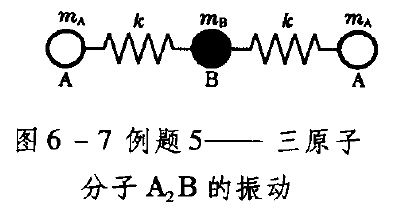
\includegraphics[width=0.5\textwidth]{image/6-7-5.JPG}
\end{figure}

\newpage

\section{振動}








\chapter{諧振子Harmonic Oscillator}
\section{彈簧振子}
\end{document}